\subsection{Discussion}

\begin{figure}[t]
\center
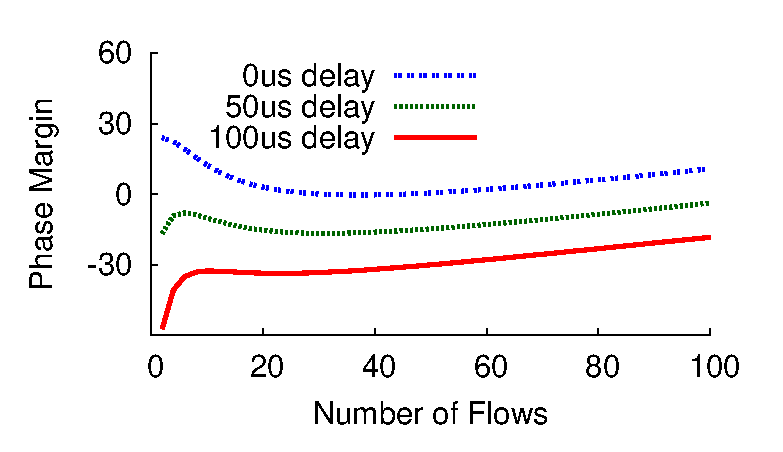
\includegraphics[width=0.4\textwidth]{figures/dcqcn_stability_100gbps.eps}
\caption{DCQCN stability with 100Gbps}
\end{figure}


\para{Extending to 100Gbps network.}  As the datacenter network fabric is moving towards 100Gbps bandwidth, we analyze
DCQCN stability given $C=100Gbps$. As shown in Figure~\ref{fig:dcqcn_100gbps}, the default parameters of DCQCN work 
reasonably well when the delay is small, {\em e.g.,} close to $0\mu s$.
However, DCQCN becomes much more sensitive to the control loop delay. With $50\mu s$ and $100\mu s$, the phase marginal
decreases much more than in 40Gbps case and leads to consistent instability.
The methods that stabilize the 40Gbps system, like tuning down $R_{AI}$ and tuning up $K_{max}$, are also effective
in 100Gbps system. We verified that with $R_{AI}=10Mbps$ and $K_{max}=1000KB$, DCQCN is stable at 100Gbps even when
the control loop delay is $100\mu s$. TODO: similar for the PI controller. We conclude that DCQCN easily adapts to 
higher bandwidth fabrics with minor tunings. 

\para{PI controller.}